\documentclass{style/modernsimplecv}
\usepackage[utf8]{inputenc}
\usepackage[top=2cm, bottom=2cm, outer=0cm, inner=0cm, margin=1cm, a4paper]{geometry}
\usepackage[sfdefault]{AlegreyaSans}
\usepackage{beuron}
\usepackage{setspace}
\usepackage{wallpaper}
\usepackage{mdframed}
\usepackage{enumitem}

\newlength{\rightcolwidth}
\newlength{\leftcolwidth}
\setlength{\leftcolwidth}{0.48\textwidth}
\setlength{\rightcolwidth}{0.47\textwidth}

\title{Curriculum Vitae}
\author{Paul Brenker}
\date{October 2024}

\pagestyle{empty}
\begin{document}
\thispagestyle{empty}

\tikz[remember picture, overlay] {%
    \node[rectangle, fill=white, anchor=north, minimum width=\paperwidth, minimum height=5cm](header) at (current page.north){};
}
% \begin{minipage}[t]{0.183\textwidth}
%     \vspace{0pt}
%     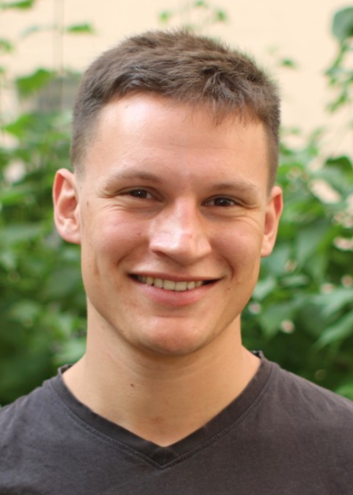
\includegraphics[width=\textwidth]{img/paul.png}\hspace{1em}
% \end{minipage}
% \hfill
\begin{minipage}[t]{0.99\textwidth} % else 80 %
    \vspace{0pt}
    \begin{shaded*}
        \begin{minipage}[t]{0.44\textwidth}
            \vspace{0pt}
            {\par\centering\huge{Paul Brenker}} \\[0.3cm]
            \faGlobe~ Nationality: German, Work Visa Israel B1\\
            \faBirthdayCake~ 1996 \\
            \faMapMarker~ Tel Aviv, Israel \\
            \begin{spacing}{0.5}
                {
                    \faCommentsO~ \underline{Languages:} \\
                    \begin{tabular}{l l}
                        \emph{German:} native & \emph{English:} full proficiency \\
                        \emph{Hebrew:} advanced proficiency & \emph{Arabic:} basic knowledge \\ 
                    \end{tabular}
                }
            \end{spacing}
            \vspace{4pt}
        \end{minipage}\hfill
        \begin{minipage}[t]{0.39\textwidth}
            \vspace{29pt} 
            \faPhone~ +972 52 3002843 \\
            \faPhone~ +49 173 5287524 \\

            \faLink~ \protect\url{www.pbrenk.com}\\
            \faAt~ \protect\url{paul.brenker@gmail.com} \\
            \faGithub~ \protect\url{github.com/paulbrenker} \\
            \faLinkedin~ \protect\url{linkedin.com/in/paul-brenker}\\
        \end{minipage}
        \hfill
    \end{shaded*}
\end{minipage}\\
\subsection*{}
\vspace{-3em}
\begin{minipage}{0.99\textwidth}
\section*{Summary}
    I am a \textbf{Computer Science} graduate Software Engineer with a great passion for deeply technical topics. Recently I moved to Israel from Germany seeking for a full-time position. My full work permit is set to be issued in September 2025 by the Israeli immigration authorities. I come with valuable experience in a thriving Software Company where I had the chance to learn and grow rapidly as the product scaled from thousands to hundreds of thousands of users.\\
    Now I am excited to start a position to take on responsibility and to really make a difference. I am eager to navigate new challenges and to work in a fast-paced environment where things get done.
\end{minipage}
\bigskip

\setlength{\columnsep}{1.7cm}
\columnratio{0.47}[0.46]
\begin{paracol}{2}
    \hbadness5000
    \paracolbackgroundoptions
    \section*{Experience}
    \begin{minipage}[t]{\leftcolwidth}
        \begin{tabular}{p{0.18\textwidth}| p{0.65\textwidth}}
            \cvevent{2023 - 2024}{SAP LeanIX}{Software Engineer - Student Position}{Bonn, Germany}{
                \vspace{-.4cm}
                \begin{itemize}[leftmargin=.3cm]    
                    \item Contributed to the LeanIX core product as part of an agile engineering team.
                    %\item Learned to work with numerous technologies used in microservice architectures.
                    \item Built backend REST service for the Architecture Decisions feature (\href{https://app.leanix.net/openapi-explorer?urls.primaryName=Documents}{Documents Service}).
                    %\item Implemented first Generative AI feature in the product portfolio summarizing To do items. and built an AI result test pipeline.
                    \item Improved performance of existing backend services by implementing cursor based pagination in combination with dynamical filtering using Spring Boot and JPA for multiple backend microservices.
                    %\item See a private demo of applied technology stack and coding practices in my own web applications: \href{}{trailmenu}, \href{}{trailmenu-frontend}
                \end{itemize}}
                {img/leanix_logo.jpg}\\

            \cvevent{2023}{LeanIX}{Intern}{Bonn, Germany}{
                \vspace{-.4cm}
                \begin{itemize}[leftmargin=.3cm]
                    \item Investigated and implemented evaluation tools for OpenAPI specifications.
                    \item Developed a prototype for a company-wide integration pipeline using GitHub Actions.
                \end{itemize}}
                {img/leanix_logo_old.jpg}\\

            \cvevent{2022 - 2023}{University of Bonn}{IT Support Student Assistant}{Bonn, Germany}{
                \vspace{-.4cm}
                \begin{itemize}[leftmargin=.3cm]
                    \item Administration of institute for philosophy websites.
                    \item Maintenance and Acquisition of IT hardware such as network devices, printers and personal computers.
                \end{itemize}}
                {img/uni_bonn_logo.png}\\

            % \cvevent{2017 - 2018}{Academy of Sciences and Humanities}{Student Assistant}{Berlin, Germany}{Transcription of ancient Hebrew and Arabic texts. XML annotation of academic text for cross-referenced usage in a database. Proofreading of articles.}{img/bbaw_logo.jpg}
        \end{tabular}
        \bigskip
        \begin{minipage}[t]{\leftcolwidth}
            \section*{Skills}
            {\normalsize

            \begin{tabular}{>{\bfseries}p{0.25\textwidth} >{}p{0.61\textwidth}}
                \textbf{Programming}  & 
                    \textbf{Java \& Kotlin for Backend},
                    \textbf{Typescript for Frontend},
                    \textbf{Python}\\
                \textbf{Frameworks} & 
                    %\textbf{Selenium},
                    \textbf{Spring Boot}, 
                    \textbf{Angular},
                    OpenAPI,
                    JPA,
                    GitHub Actions, 
                    PostgreSQL\\
                \textbf{Technologies} & 
                    \textbf{AWS (certified)},
                    \textbf{Linux Server \& Desktop},
                    \textbf{REST APIs},  
                    Databases, 
                    Git, 
                    Docker, 
                    Data Analysis, 
                    Machine Learning, 
                    LaTeX\\
                \textbf{Methodologies} & 
                    \textbf{Technical Documentation},
                    \textbf{TDD},
                    \textbf{CI/CD},
                    %Functional Programming, 
                    Agile, 
                    Microservices\\
            \end{tabular} 
            }

        \end{minipage}\hfill
    \end{minipage}
    \switchcolumn
    \bigskip
    \begin{minipage}[t]{\rightcolwidth}
        \section*{Education}
        \begin{tabular}{p{0.18\textwidth}| p{0.65\textwidth}}
            \cvevent{2019 - 2024}{Bonn-Rhein-Sieg University of Applied Sciences (H-BRS)}{B.S. Computer Science}{Bonn, Germany}{
                \vspace{-.4cm}
                \begin{itemize}[leftmargin=.3cm]
                    \item Computer Science degree with a final grade of 1.6 GPA (German) (=90 \% (Israeli)) within the best 10 \% of faculty graduates.
                    \item Specialized in Bioinformatics and Data Science where I did multiple applied projects. (E.g. \href{https://github.com/paulbrenker/decision-tsp}{github.com/paulbrenker/decision-tsp})
                    \item For my Thesis I chose the topic: Relevance of OpenAPI Linter Rules for Specification Quality. (\href{https://github.com/paulbrenker/thesis}{github.com/paulbrenker/thesis})
                \end{itemize}}
                {img/hbrs_logo.jpg} \\
                
            \cvevent{2015 - 2019}{Freie Universität zu Berlin}{B.A. Linguistics}{Berlin, Germany}{
                \vspace{-.4cm}
                \begin{itemize}[leftmargin=.3cm]
                    \item Focused on Middle Eastern languages including Hebrew, Arabic, Amharic and Aramaic.
                    \item Abroad stays in Egypt, Israel and Jordan.
                    \item Thesis was written about gender-specific variations in the Arabic dialect of Amman, Jordan. 
                \end{itemize}}
                {img/fu_logo.png} \\
        \end{tabular}
    \bigskip
    \begin{minipage}[t]{\rightcolwidth}
        \section*{Scholarships}
        \begin{tabular}{>{\bfseries}p{0.12\textwidth} >{}p{0.7\textwidth}}
            2023 & Deutschlandstipendium - Scholarship for ambitious and talented students                                                  \\
            2018 & Scholarship for a full Semester of intensive Arabic language courses at the German Jordanian University in Amman, Jordan. \\
            2018 & PROMOS -  Scholarship for an intensive Hebrew summer school at the Ben Gurion University of the Negev                     \\
        \end{tabular}
    \end{minipage}\hfill
    \bigskip
    \begin{minipage}[t]{\rightcolwidth}
        % \section*{Volunteering}
        % \begin{tabular}{>{\bfseries}p{0.12\textwidth} >{}p{0.7\textwidth}}
        %     2014 & After graduating from high school I volunteered for nine months in Kibbutz Ein Hashlosha in Israel. During my time I worked mostly in agriculture and landscaping but also in the local garage where I helped to maintain the vehicles of the Kibbutz. \\
        % \end{tabular}
        % \bigskip
        \section*{Hobbies}
        \begin{tabular}{>{\bfseries}p{0.12\textwidth} >{}p{0.7\textwidth}}
            Rowing  & I row since I am ten years old and participated in countless competitions including the German national sprint league. \\
            Cycling & I love to ride bicycles not just for sport but also in the everyday for a sustainable and balanced life.
        \end{tabular}
    \end{minipage}
\end{minipage}
\end{paracol}

%\vfill{} % Whitespace before final footer
% \setlength{\parindent}{0pt}
% \begin{minipage}[t]{\textwidth}
%     \begin{center}\fontfamily{\sfdefault}\selectfont \color{black!70}
%         {\small Paul Brenker 
%         %\icon{\faEnvelopeO}{black}{} Maxstr. 28 
%         \icon{\faMapMarker}{black}{} Tel Aviv 
%         \icon{\faPhone}{black}{} +972 52 3002843
%         \icon{\faPhone}{black}{} +49 173 5287524
%         \icon{\faAt}{black}{} \protect\url{paulbrenker@gmail.com}
%         }
%     \end{center}
% \end{minipage}
\end{document}